\chapter{Burglar's Night Out}

\section{Problem Statement}

A burglar has come to your neighborhood at night. Your neighborhood has many houses arranged in a linear fashion and each house has some amount of money. The burglar wishes to take as much money as possible. However, he cannot rob two consecutive houses otherwise the security bell will ring and he will get caught.

\begin{figure}[H]
    \centering
    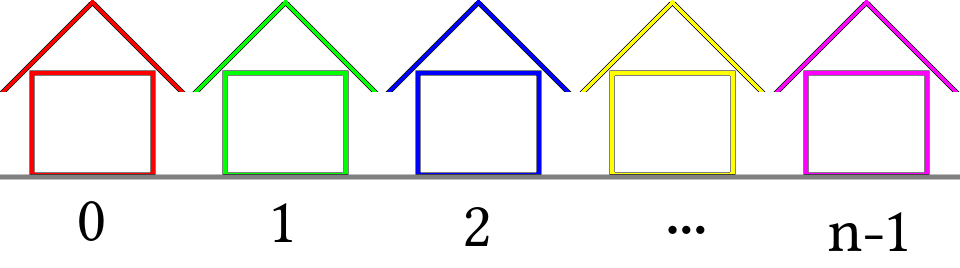
\includegraphics[width=\textwidth]{images/blurglars_night_out/houses.png}
\end{figure}

\section{Basic Definitions}

\newcommand{\binarySet}{\ensuremath{\mathbb{B}}}
\renewcommand{\cost}[2]{\ensuremath{\apply{\sigma_{#2}}{#1}}}

\begin{defn}[Binary Sequence and Real Sequence]
    A \textbf{Binary Sequence} is a sequence of values of the binary set $\binarySet = \Set{True, False}$.
    A \textbf{Real Sequence} is a sequence of values of the real set $\R$.
\end{defn}

\begin{defn}[Cost of a Sequence]
    Given a Binary Sequence $b$ and a real sequence $r$, both with the same length, the \textbf{Cost $\cost{b}{r}$ of the Sequence $b$} with values $r$ is given by:
    \begin{equation}
        \cost{b}{r} = \Sum{i \in \SetOf{i \in \range{n}}{b[i] = True}}{}{r[i]}
    \end{equation}
\end{defn}

\begin{defn}[True Alternate Binary Sequence]
    A Binary Sequence $b$ is called \textbf{True Alternate Binary Sequence} or simply \textbf{True Alternate} if there are no two consecutive values in which both are $True$. In other words:
    \begin{align}
        & \forall i \in \range{n} \nexists j \in \range{n} \left(
            j = i + 1
            \land
            i = True
            \land
            j = True
        \right)
        & \equiv \\\nonumber
        &
        \forall i \Big(
            \left(i \in \range{n} \land i = True\right)
            \rightarrow
            \nexists j \left(
                j \in \range{n}
                \land
                j = i + 1
                \land
                j = True
            \right)
        \Big) &
    \end{align}
\end{defn}

\section{Problem Definition}

\begin{enumerate}
    \item Input:
    \begin{enumerate}
        \item the number of houses: a natural number $n \in \N$;
        \item the value sequence: a Real Sequence $r$ of length $n$;
    \end{enumerate}
    \item Output: a True Alternate Binary Sequence $b$ of length $n$;
    \item Goal: Maximize the cost of the sequence $\cost{b}{r}$;
\end{enumerate}

\section{Naive Algorithm}

\begin{algorithm}[H]
    \caption{Naive}
    \label{burglar's-night-out:algorithm:naive}
    \begin{algorithmic}[1]
        \Require{$n \in \N, r \in \R^n$}
        \State{$S \gets \mbox{generate\_all\_binary\_sequences}(n)$}
        \State{$S' \gets \mbox{filter\_true\_alternate\_sequences}(S)$}
        \State{$s^* \gets \ArgMax{s \in S'}{\cost{s}{r}}$}
        \State{\textbf{return} $s^*$}
    \end{algorithmic}
\end{algorithm}
